% Chapter 3

\chapter{Background} % Main chapter title here

\label{Chapter3} % For referencing the chapter elsewhere, use \ref{Chapter3}

\lhead{Chapter 3. \emph{Background}} % This is for the header on each page perhaps a shortened title


\definecolor{mygreen}{rgb}{0,0.6,0}
\definecolor{mygray}{rgb}{0.9,0.9,0.9}
\definecolor{mymauve}{rgb}{0.58,0,0.82}
\definecolor{mybrown}{RGB}{178,34,34}

%\frametitle{Inserting source code without setting typewriter}
\lstset{language=C++,
  backgroundcolor=\color{mygray},
  numbers=left,                    % possible val ues are (none, left, right)
  numbersep=-8pt,                   % how far the line-numbers are from the code
  numberstyle=\tiny\color{mybrown}, % the style that is used for the line-numbers
  stepnumber=1,                    % each line will be numbered
  morekeywords={*},
  keywordstyle=\color{blue},
  stringstyle=\color{mymauve},
  commentstyle=\color{mygreen},
  morecomment=[l][\color{magenta}]{\#},
  basicstyle=\footnotesize,        % the size of the fonts that are used for the code
  keepspaces=false,                 % keeps spaces in text, useful for keeping indentation of code
  columns=flexible,
  breaklines=true
  rulesepcolor=\color{mygray},
  rulecolor=\color{mygray}
}
%----------------------------------------------------------------------------------------
In this chapter, some important technical backgrounds will be covered. First it explains the \textit{CPE WAN Management Protocol (CWMP)} which defines several data models. Then is the Mios which is the main partner of Orange on the Smart Home project. Also the \textit{NAT traversal} will be presented after Mios, it is a computer networking methodology with the goal to establish and maintain Internet protocol connections across gateways that implement \textit{network address translation (NAT)}.At last, the Homelive box will be analysed, including the HardWare analyse, operating system OpenWRT and Cross-Compiling between working machine and the embedeed system OpenWRT.

\section{CWMP}

CPE WAN Management Protocol (CWMP) is a technology specification initiated and developed by the Digital Subscriber’s Line DSL Forum(now Broadband Forum). CWMP is numbered TR-069 by the forum and is thus also called the TR-069 protocol. It defines the general frame, message format, management method, and data model for the management and configuration of home network devices in next-generation networks.

CWMP is mainly applied to DSL access networks, which are hard to manage because user devices are located at the customer premise, dispersed, and large in number. CWMP makes the management easier by using an auto-configuration server (ACS) to perform remote centralized management of customer premises equipment (CPE).



\subsection{CWMP Protocol}
\label{basics}
CWMP is a text based protocol. Orders sent between the device (CPE) and auto configuration server (ACS) are transported over HTTP (or more frequently HTTPS)(\fref{fig:remotecontrol}). At this level (HTTP) CPE is behaving in the role of client and ACS in the role of HTTP server. This essentially means that control over the flow of the provisioning session is the sole responsibility of the device.
\begin{figure}[htbp]
	\centering
		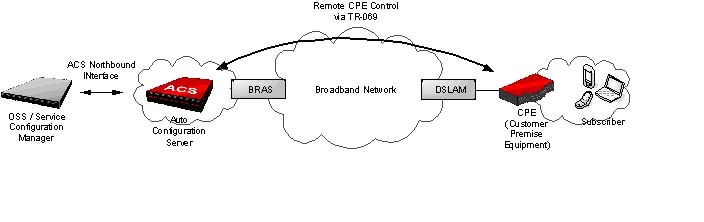
\includegraphics[width=9.5cm]{Figures/Remote_CPE_Control_via_TR-069.jpg}
	\caption[Remote CPE Control via TR-069]{Remote CPE Control via TR-069}
	\label{fig:remotecontrol}
\end{figure}
%-------------------------------------------------------
\subsubsection{Provisioning session}
All communications and operations are performed in the scope of the provisioning session. The session is always started by the device(CPE) and begins with the transmission of an Inform message. Its reception and readiness of the server for the session is indicated by an InformResponse message. That concludes the session initialization stage. The order of the next two stages depends on the value of the flag HoldRequests. If the value is false the initialization stage is followed by the transmission of device requests, otherwise ACS orders are transmitted first. The following description assumes the value is false.

In the second stage, orders are transmitted from the device to the ACS. Even though the protocol defines multiple methods that may be invoked by the device on the ACS, only one is commonly found - TransferComplete which is used to inform the ACS of the completion of a file transfer previously issued Download or Upload request. This stage is finalized by transmission of empty HTTP-request to the ACS.

In the third stage the roles change on the CWMP level. The HTTP-response for the empty HTTP-request by the device will contain a CWMP-request from the ACS. This will subsequently be followed by an HTTP-request containing a CWMP-response for the previous CWMP-request. Multiple orders may be transmitted one-by-one. This stage (and the whole provisioning session) is terminated by an empty HTTP-response from the ACS indicating that no more orders are pending.



\subsubsection{Security and authentication}
As vital data (like user names and passwords) may be transmitted to CPE via CWMP, it is essential to provide secure transport channel and always authenticate the CPE against the ACS. Secure transport and authentication of the ACS identity can easily be provided by usage of HTTPS and verification of ACS certificate. Authentication of the CPE is more problematic. The identity of the device is verified based on a shared secret (password) at the HTTP level. Passwords may be negotiated between the parties (CPE-ACS) at every provisioning session. When the device contacts the ACS for the first time (or after a factory-reset) default passwords are used. In large networks it is the responsibility of the procurement to ensure each device is using unique credentials, their list is delivered with the devices themselves and secured.


\subsubsection{Connection request}

The following example\fref{fig:connectionrequest} illustrates how CWMP works. The scenario: There are two ACSs, active and standby in an area. The active ACS needs to restart for system upgrade. To ensure a continuous monitoring of the CPE, the active ACS needs to let all the CPE in the area connect to the standby ACS. The whole process is as follows:

\begin{figure}[htbp]
	\centering
		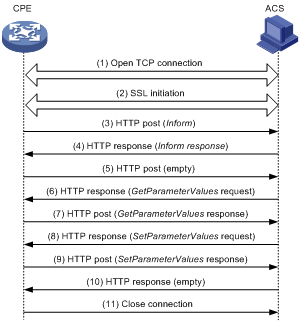
\includegraphics[width=9.5cm]{Figures/connection_request.png}
	\caption[CWMP Connection Scenario]{CWMP Connection Scenario}
	\label{fig:connectionrequest}
\end{figure}

\begin{enumerate}
  \item Establish a TCP connection
  \item SSL initiation, and establish a security mechanism
  \item The CPE sends an Inform request message to initiate a CWMP connection. The Inform message carries the reason for sending this message in the Eventcode field. In this example, the reason is “6 CONNECTION REQUEST”, indicating that the ACS requires the CPE to establish a connection.
  \item If the CPE passes the authentication of the ACS, the ACS returns an Inform response, and the connection is established.
  \item Receiving the Inform response, the CPE sends an empty message if it has no other requests. The CPE does this in order to comply with the request/reply interaction model of HTTP, in which CWMP messages are conveyed.
  \item The ACS queries the value of the ACS URL set on the CPE.
  \item The CPE replies the ACS with the obtained value of the ACS URL.
  \item The ACS finds that its local URL value is the same as the value of the ACS URL on the CPE. Therefore, the ACS sends a Set request to the CPE to modify the ACS URL value of the CPE as the URL of the standby ACS.
  \item The setting succeeds and the CPE sends a response.
  \item The ACS sends an empty message to notify the CPE that it has no other requests.
  \item The CPE closes the connection.
\end{enumerate}

After this, the CPE will initiate a connection to the standby ACS.

\subsubsection{CR over NAT}
The CWMP protocol also defines a mechanism for reaching the devices that are connected behind NAT (e.g. IP-Phones, Set-top boxes). This mechanism, based on STUN and UDP NAT traversal, is defined in document TR-069 Annex G (formerly in TR-111).

Amendment 5 of the protocol introduces alternative method of executing Connection Request via NAT based on XMPP (see Annex K of TR-069 Amendment 5 for details).


\subsection{Data Model}
The Broadband Forum defines several data models for use with the CPE WAN Management Protocol (TR-069 Amendment 5). These data models contain objects and parameters that describe the many different functions and capabilities available to devices and services that are manageable via CWMP.

CWMP data models are divided into two types: Root and Service. The root data model, Device1, is used to describe the major functions of a network aware device, including interfaces, software/firmware, diagnostics, components common to CWMP and other services, and the basic device information necessary to CWMP.

Service data models describe modular functionality that allow the extension of the root data model on a device (under Device.Services.) to provide particular services, such as a voice service, set top box service, network attached storage, etc.

Each data model is defined by a Name:Version syntax. A device defines its data model by defining a device type, an XML document that maps to (imports) BBF official data model objects and/or vendor specific objects. A full explanation of how to develop compliant CWMP data models can be found in TR-154.

%--------------------------------------
Most of the configuration and diagnostics is performed through setting and retrieving the value of the device parameters. These are organized in a well defined hierarchical structure that is more or less common to all device models and manufacturers. Broadband Forum publishes its data model standards in two formats - XML files containing a detailed specification of each subsequent data model and all of the changes between their versions and PDF files containing human-readable details. Supported standards and extensions should be clearly marked in the device data model. This should be in the field Device.DeviceSummary or InternetGatewayDevice.DeviceSummary which is required starting from Device:1.0 and InternetGatewayDevice:1.1 respectively. If the field is not found InternetGatewayDevice:1.0 is implied. As of Device:1.4 and InternetGatewayDevice:1.6 new field ( \'<RO>\'.SupportedDatamodel) for supported standard specification was introduced.

The model is always rooted in the single key named Device or InternetGatewayDevice depending on the manufacturer's choice. At each level of the structure objects and parameters (or array-instances) are allowed. Keys are constructed by concatenating the names of objects and parameter using '.'(dot) as a separator, e.g. InternetGatewayDevice.Time.NTPServer1 .

Each of the parameters may be marked as writable or non-writable. This is reported by the device in GetParameterNamesResponse message. The device should not permit the change of any parameter marked as read-only. Data model specifications and extensions clearly mark required status of most of the parameters.

Values applicable for the parameter, their type and meaning are also precisely defined by the standard.

\textbf{Multi-instance objects} :Some parts of the data model require the existence of multiple copies of the subtree. The best examples are those describing tables, e.g. Port Forwarding Table. An object representing an array will only have instance numbers or alias names as its children.

A multi-instance object may be writable (enabling dynamic creation and/or removal of its children) or read-only depending on the data represented. If for example the object represents four physical ports on a switch it should not be possible to add or remove them from the data model. If an instance is added to an object an identifier is assigned. After being assigned, identifiers may not change during the life-cycle of the device except for factory-reset.
%------------------------------------------------------------------------------------------------------------
\section{Mios}
MiOS, LTD. is a global software and hardware company represented in over 60 countries, and focused on developing and distributing advanced control and monitoring solutions for the home and small enterprise markets. Founded in 2008, MiOS has created the technology platform that bridges many different devices to produce hardware and software solutions for home control networks. Now in its fifth generation, the MiOS platform allows users to remotely control, monitor and automate their households and businesses with products that are currently available from any vendor.

At January 6th, 2014. MiOS has been selected as the platform partner for Orange’s Smart Home initiative. This announcement followed a successful launch with MiOS as the platform for Orange Poland’s Smart Home program.  The Orange initiative will be initially offered in several countries in Europe.

\subsection{Luup}
Luup (Lua-UPnP) is Mi Casa Verde(Mios)’s new software engine which incorporates \textit{Lua}, a popular scripting language, and \textit{UPnP}, the industry standard way to control devices. Vera is built on Luup.

On this platform, since the API includes drivers for Z-Wave, Insteon, etc., and talks to infrared and serial devices, home automation is the first thing that we can do on Luup. However Lua is a full-featured language and not limited just to scripting. Also, we can write modules in C/C++ that run on Vera, which the main Luup engine will also aggregate and control.

\subsection{MMS}
MMS is the management platform based on http request. To be able to use the MMS, we have to authenticate to a valid user of an account:

Here is a login example:
\begin{lstlisting}[mathescape]
	https://orangefut-autha1.com/autha/auth/username/bob?SHA1Password=86e739edcc&PK_Oem=33
\end{lstlisting}

And the body of the response (Identity and IdentitySignature are truncated):

\begin{lstlisting}[mathescape]
    "Identity": "eyJFeHBpcmVzIjoxNDAw...YW5nZV9tYXN0ZXIifQ==",
    "IdentitySignature": "L5H6babTjsZwk7RiAeRP...W91tWSMIbI9x7jJmsQ==",
    "Server_Event": "orangefut-event12.com",
    "Server_Event_Alt": "orangefut-event11.com",
    "Server_Account": "orangefut-account12.com",
    "Server_Account_Alt": "orangefut-account11.com"
\end{lstlisting}
%----------------------------------------------------------------------------------------------------------------
\section{NAT Traversal}
NAT traversal is a computer networking methodology with the goal to establish and maintain Internet protocol connections across gateways that implement network address translation (NAT). NAT breaks the principle of end-to-end connectivity originally envisioned in the design of the Internet.

NAT traversal techniques are required for certain client-to-client network applications, such as peer-to-peer file sharing and Voice over IP.\cite{stiemerling2008nat}

%----------------------------------------------------------------------------------------------------------------

\subsection{Principals}

Many techniques exist, but no single method works in every situation since NAT behavior is not standardized. Many NAT traversal techniques require assistance from a server at a publicly routable IP address\cite{rosenberg2003stun}. Some methods use the server only when establishing the connection, while others are based on relaying all data through it, which adds bandwidth costs and increases latency, detrimental to real-time voice and video communications.

NAT devices are commonly used to alleviate IPv4 address exhaustion\cite{alqahtaniipv4} by allowing the use of private IP addresses on home and corporate networks behind routers with a single public IP address facing the public Internet. The internal network devices communicate with hosts on the external network by changing the source address of outgoing requests to that of the NAT device and relaying replies back to the originating device.

The NAT traversal techniques available are as following:
\begin{itemize}
  \item \textit{Socket Secure (SOCKS)} is a technology created in the early 1990s that uses proxy servers to relay traffic between networks or systems.
  \item \textit{UPnP IGD} is supported by many small NAT gateways in home or small office settings.
  \item \textit{Interactive Connectivity Establishment (ICE)} is a technique used in VoIP, peer-to-peer communications, video, instant messaging, and other interactive media applications. It uses Session Traversal Utilities for NAT (STUN).
  \item \textit{Application-level gateway (ALG)} is a component of a firewall or NAT that allows for configuring NAT traversal filters.\cite{hu2005nat}
  \item \textit{NAT hole punching} is a technique that exploits how NATs handle some protocols (for example, UDP, TCP, or ICMP) to allow previously blocked packets through the NAT.
\end{itemize}

At Orange Labs, we use \textit{UPnP IGD} and \textit{STUN}to manage NAT traversal.
%----------------------------------------------------------------------------------------------------------------
\subsection{UPnP IGD}

Universal Plug and Play (UPnP)\cite{jeronimo2003upnp} is a set of networking protocols that permits networked devices, such as personal computers, printers, Internet gateways, Wi-Fi access points and mobile devices to seamlessly discover each other's presence on the network and establish functional network services for data sharing, communications, and entertainment. UPnP is intended primarily for residential networks without enterprise-class devices.

The UPnP technology is promoted by the UPnP Forum, a computer industry initiative to enable simple and robust connectivity to stand-alone devices and personal computers from many different vendors. The Forum consists of over eight hundred vendors involved in everything from consumer electronics to network computing.

The concept of UPnP is an extension of plug-and-play, a technology for dynamically attaching devices directly to a computer, although UPnP is not directly related to the earlier plug-and-play technology. UPnP devices are "plug-and-play" in that when connected to a network they automatically establish working configurations with other devices.

Internet Gateway Device (IGD) Standardized Device Control Protocol is a protocol for mapping ports in network address translation (NAT) setups, supported by a certain number of NAT-enabled routers.\cite{wing2013p} It is a common communications protocol of automatically configuring port forwarding, and is part of an ISO/IEC Standard \cite{sherwin2009upnp} rather than an Internet Engineering Task Force standard.

Applications using peer-to-peer networks, multiplayer gaming, and remote assistance programs need a way to communicate through home and business gateways. Without IGD one has to manually configure the gateway to allow traffic through, a process which is error prone and time consuming. Universal Plug and Play (UPnP) comes with a solution for network address translation traversal.

IGD makes it easy to do the following:

\begin{itemize}
  \item Learn the public (external) IP address
  \item Requesting for a new public IP address\cite{srisuresh1999ip}
  \item Enumerate existing port mappings
  \item Add and remove port mappings
  \item Assign lease times to mappings
\end{itemize}
%----------------------------------------------------------------------------------------------------------------
\subsection{STUN}
STUN (Session Traversal Utilities for NAT) is a standardized set of methods and a network protocol to allow an end host to discover its public IP address if it is located behind a NAT. It is used to permit NAT traversal for applications of real-time voice, video, messaging, and other interactive IP communications. It is documented in RFC 5389\cite{rosenberg2008rfc}. The STUN URI scheme is documented in RFC 7064. STUN is intended to be a tool to be used by other protocols, such as ICE.

The STUN protocol allows applications operating behind a network address translator (NAT) to discover the presence of the network address translator and to obtain the mapped (public) IP address (NAT address) and port number that the NAT has allocated for the application's User Datagram Protocol (UDP) connections to remote hosts. The protocol requires assistance from a third-party network server (STUN server) located on the opposing (public) side of the NAT, usually the public Internet.


\begin{figure}[htbp]
	\centering
		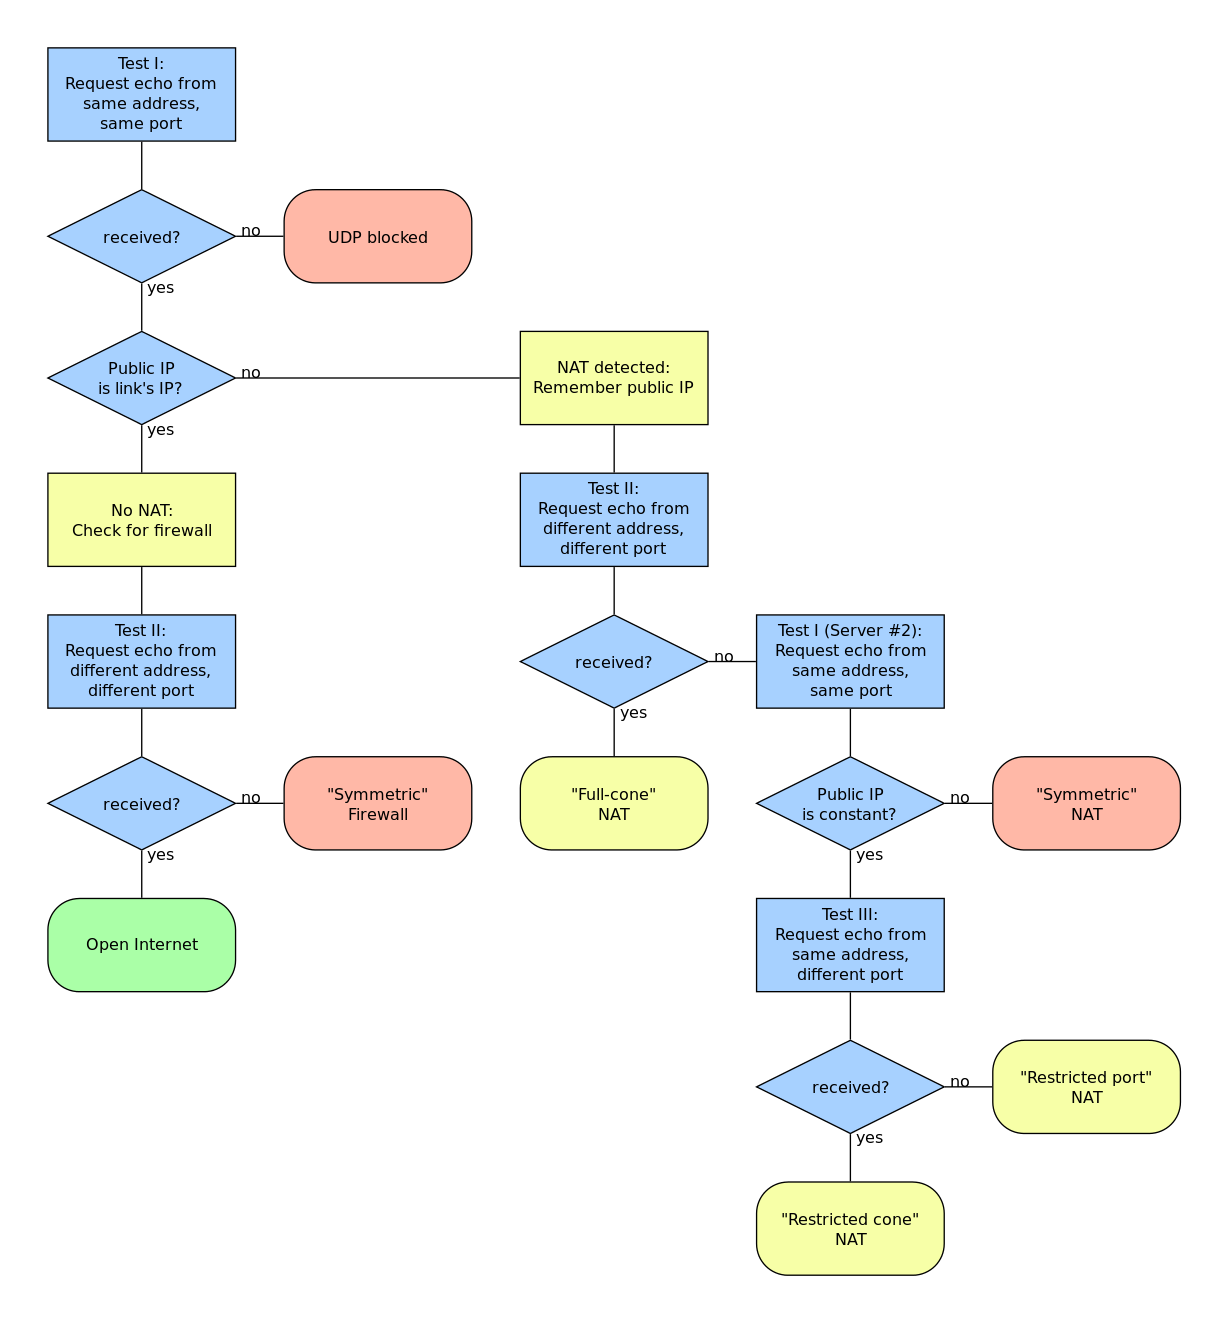
\includegraphics[width=9.5cm]{Figures/STUN_Algorithm.png}
	\caption[STUN Algorithm to track the Public Address]{STUN Algorithm to track the Public Address}
	\label{fig:stunalgorithm}
\end{figure}
%----------------------------------------------------------------------------------------------------------------
\section{Homelive Box}
Homelive is the Smart Home set-top box of Orange, which is the center of the Z-Wave network.

%----------------------------------------------------------------------------------------------------------------
\subsection{Hardware}

\begin{figure}[htbp]
	\centering
		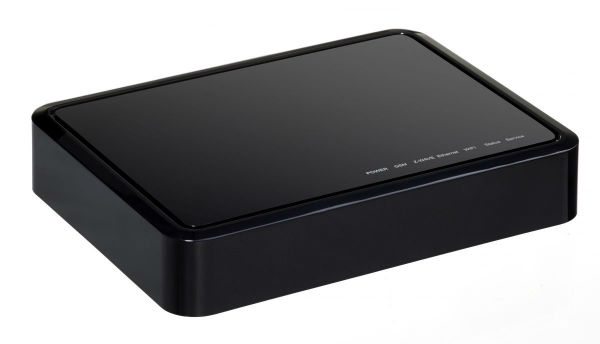
\includegraphics[width=9.5cm]{Figures/Orange-Home-Live.jpg}
	\caption[Homelive Box of Orange]{Homelive Box of Orange}
	\label{fig:homelivebox}
\end{figure}

Here is the list of Homelive components:

\begin{center}
  \begin{tabular}{@{} cc @{}}
    \toprule
    Item & Value \\*
    \midrule
    Architecture & MIPS64 \\
    Operating System & OpenWRT BarrierBreaker 14.07\\
    Firmware & Luup (Lua \& UPnP) \\
		Processeur & MT7620A (580 MHz) \\
		Capacité mémoire & 128 MB DDR2, 128 MB capacité flash NAND \\
		Connectivité Cellulaire & 2G quad bandes \\
		Connectivité RF & Z-Wave Serie 500 \\
		Connectivité Wi-Fi & 2.4 GHz 11n 2x2 \\
		Connectivité réseau & 1 port RJ45 10/100 \\
		Connectivité multimédia & 1 port USB2.0 \\
		Carte Sim & 1 Slot externe \\
		Dimensions & 174 mm x 129 mm x 33 mm (L x l x h) \\
		Poids & 421 g \\
		Alimentation externe & 12 V \\
		Consommation électrique & 3 W \\
    \bottomrule
  \end{tabular}
%	\caption[Homelive Box of Orange]{Homelive Box of Orange}
\end{center}

The MIPS64 architecture is based on a fixed-length, regularly encoded instruction set, and it uses a load/store data model. It is streamlined to support optimized execution of high-level languages. Arithmetic and logic operations use a three-operand format, allowing compilers to optimize complex expressions formulation. Availability of 32 general-purpose registers enables compilers to further optimize code generation by keeping frequently accessed data in registers.
%----------------------------------------------------------------------------------------------------------------
\subsection{OpenWRT}
OpenWrt\cite{fainelli2008openwrt} is a highly extensible GNU/Linux distribution for embedded devices (typically wireless routers). Unlike many other distributions for these routers, OpenWrt is built from the ground up to be a full-featured, easily modifiable operating system for your router. In practice, this means that you can have all the features you need with none of the bloat, powered by a Linux kernel that's more recent than most other distributions. The main components are the Linux kernel, util-linux, uClibc or musl, and BusyBox. All components have been optimized for size, to be small enough for fitting into the limited storage and memory available in home routers.

OpenWrt is configured\cite{petullo2010building} using a command-line interface (ash shell), or a web interface (LuCI). There are about 3500 optional software packages available for installation via the opkg package management system.

OpenWrt can run on various types of devices, including \textit{CPE routers}, residential gateways, smartphones (e.g. Neo FreeRunner), pocket computers (e.g. Ben NanoNote), and laptops (e.g. One Laptop per Child (OLPC)). It is also possible to run OpenWrt on ordinary computers, which are most commonly based on the x86 architecture. Many patches from the OpenWrt's codebase have been included upstream in the Linux kernel mainline.
%----------------------------------------------------------------------------------------------------------------
\subsection{Cross-Compiling}

Cross compiling is the process that capable of creating executable code for a platform other than the one on which the compiler is running. For example, a compiler that runs on a Windows 7 PC but generates code that runs on Android smartphone is a cross compiler.

In our case, in the reason of the source of hardware in Homelive is very limited, we should finish the compilation of source code under the Linux Machine. To archieve this, we should get prepared with the compile tool chain which is provided by OpenWRT. The steps are:

\begin{enumerate}
  \item Download OpenWRT package prom officail site
  \item Compile OpenWRT on Linux machine and select the packages needed for Homelive Box
  \item Generate the tool-chain of compilation
  \item Comple the TR-069 source code with OpenWRT tool chain
  \item Transfer excutable files to Homelive
\end{enumerate}

The disadvantage of cross compiling is that we can\'t use debug tools like \textit{GDB}.
